\documentclass[11pt,fontset=none]{ctexart}
\setCJKmainfont{SimSun}[BoldFont=SimHei]
\setCJKsansfont{Microsoft YaHei}
\setCJKmonofont{SimHei}
\usepackage[margin=1in]{geometry}
\usepackage{booktabs}
\usepackage{longtable}
\usepackage{graphicx}
\usepackage{hyperref}

\title{在虚拟机上复现 LEBench\\
\large Linux 核心操作性能演化分析}
\author{邹浩宇 \quad 5260000157\\
CS340 操作系统，2026--2027}
\date{2026年11月3日}

\begin{document}
\maketitle

本文与英文版 \texttt{report/report.tex} 使用同一批客户机日志。表中的测试名与 CSV 中的名字一致，其中上下文切换在作者代码里写成 \texttt{context siwtch}。

\section{引言与论断}

Ren 等人测量了 Linux 3.0 到 4.20 上核心操作的延迟，认为内核变慢了，主要原因是安全补丁、新功能，以及少量配置错误 \cite{ren2019lebench}。这些操作就是 LEBench 直接计时的项目：\texttt{getpid}、上下文切换、fork、读/写、mmap/munmap、缺页、send/recv，以及 select/poll/epoll。

论文里有三条论断：

\begin{enumerate}
\item \textbf{图 1(a)。} 相对 Linux 4.0，更晚的内核在这些操作上更慢，大块写和大块 munmap 除外。多数测试也比 3.0 更慢，而且很多至少慢 50\%。
\item \textbf{表 3 与图 2。} 十一个改动解释了大幅跳动。其中四个是安全补丁，四个是新功能，三个是配置错误。
\item \textbf{第 5 节。} 关掉这十一项之后，Redis、Apache 和 Nginx 最多分别加快 56\%、33\% 和 34\%。
\end{enumerate}

这次复现检验作者实验笔记里那份内核清单上的论断 1，并把论断 2 里的一个因素（页表隔离）当作扩展实验。论断 3 没有跑。作者的 \texttt{EXPERIMENTS.md} 列出了 41 个 Ubuntu 主线版本，从 3.0.7 到 4.20.13。论文正文写的是 36 个版本。驱动程序对这份清单里的每一个版本都做了尝试。

\section{复现设置}

\subsection{起点代码}

基准程序是作者的 LEBench，提交 \texttt{6aa7801}（\url{https://github.com/LinuxPerfStudy/LEBench}），Apache-2.0，版权 2019 年多伦多大学。\texttt{TEST\_DIR/OS\_Eval.c}、\texttt{run.py} 和 \texttt{get\_kern.py} 没有改。课程用的运行程序是 \texttt{course/OS\_Eval\_reduced.c}，由 \texttt{course/make\_reduced\_eval.py} 从原文件生成。它保留同样的 \texttt{clock\_gettime} 区间和同样的 K-best 规则（五个样本落在 5\% 以内）。\texttt{BASE\_ITER} 从 10{,}000 改成 40，去掉了 60 秒的静置，并且不编译三项会阻塞或占满运行时间的测试：96\,KB 的 send/recv、12{,}000 页的 fork，以及 10{,}000 页的文件测试。在嘈杂的虚拟机上，原程序遇到空的 K-best 结果会退出；这里改成退回到最小的那次样本。

另一份用 \texttt{rdtsc} 重写测试的代码没有用来出数。原因见第~\ref{sec:rewrite} 节。

\subsection{环境}

\begin{center}
\begin{tabular}{@{}ll@{}}
\toprule
项目 & 设置 \\
\midrule
宿主机 & Windows 11，第 13 代 Intel Core i7-13700H \\
虚拟机 & VirtualBox 7.2.22，传统 BIOS，NAT \\
客户机 & Ubuntu 16.04.6 LTS，英文 \\
资源 & 2 个虚拟 CPU，4\,GB 内存，80\,GB 磁盘，位于 \texttt{D:} \\
编译器 & gcc 5.4.0（\texttt{-O0 -pthread}，与上游 makefile 相同） \\
恢复用内核 & 4.4.0-210-generic，只用来安装和恢复 \\
\bottomrule
\end{tabular}
\end{center}

宿主机开了内存完整性，VirtualBox 不能走它的快速虚拟化路径。客户机看到的 CPU 型号字符串仍然是宿主机的 i7-13700H。这颗 CPU 对 Meltdown 的报告是“Not affected”。

\subsection{工作负载}

每个启动成功的内核都以 root 运行三次 \texttt{course/sweep\_bench}。这个二进制文件就是精简后的 \texttt{OS\_Eval}。它写出作者原来的 CSV：每个测试一行 K-best、一行平均值，单位是秒。报告里的数字是三次 K-best 的均值和样本标准差。日志在 \texttt{results/kernels/<版本>/runN.csv}，另外还有标准输出、标准错误、退出码和 \texttt{environment.txt}。

内核包来自作者的备份仓库 \url{https://github.com/LinuxPerfStudy/ExperimentSetup}，目录 \texttt{default\_ubuntu\_kernels}。驱动程序下载 \texttt{linux-image} 的 deb（如果只有 unsigned 包，就用 unsigned），装上之后用 \texttt{grub-reboot} 指定下一次启动。如果 panic，下一次开机回到 4.4.0-210。没有对分区执行上游的 \texttt{grub-install}。

\subsection{与论文的差别}

\begin{center}
\small
\begin{tabular}{@{}p{0.18\linewidth}p{0.26\linewidth}p{0.24\linewidth}p{0.22\linewidth}@{}}
\toprule
项目 & 论文 & 本次 & 原因 \\
\midrule
机器 & HP DL160 G9，Xeon E5-2630 v3，128\,GB，SSD & i7-13700H 上的 VirtualBox，2 个 vCPU，4\,GB & 没有那台服务器。比较只在同一台客户机内进行。 \\
内核数量 & 正文写 36 个版本 & 作者列出的全部 41 个版本 & 发布出来的清单才是可以复现的集合。 \\
迭代次数 & \texttt{BASE\_ITER} 为 10{,}000，并静置 60 秒 & \texttt{BASE\_ITER} 为 40，不静置 & 在这台客户机上，完整一轮要几个小时。K-best 规则没有改。 \\
省掉的测试 & 96\,KB 的 send/recv、12{,}000 页的 fork、10{,}000 页的 I/O & 不编译进去 & 上游注释写明大块 send 在旧内核上会阻塞。另外两项占满运行时间。 \\
统计量 & 进程内的 K-best & 先取该值，再对 3 个进程做均值 $\pm$ 样本标准差 & 课程要求报告跨次运行的统计量。 \\
应用程序 & Redis、Apache、Nginx & 没有跑 & 先做论断 1 和一项安全开关。 \\
\bottomrule
\end{tabular}
\end{center}

\section{结果}

\subsection{已安装内核上的页表隔离}
\label{sec:ext}

这次对照只改一个因素。内核 4.4.0-210-generic 启动两次：一次用默认命令行，一次在同一内核上加上 \texttt{nopti}。硬件、二进制和迭代次数都不变。两次启动里，\path{/sys/devices/system/cpu/vulnerabilities/meltdown} 都是“Not affected”。Spectre v2 保持 Enhanced IBRS。

表~\ref{tab:nopti} 由 \texttt{scripts/render\_results.py} 根据 \texttt{results/kernel\_summary.csv} 算出。“重叠”表示两个“均值 $\pm$ 标准差”区间相交。

\begin{table}[ht]
\centering
\caption{同一内核、同一二进制。默认命令行对照 \texttt{nopti}。各三次。}
\label{tab:nopti}
\begin{tabular}{@{}lrrrr@{}}
\toprule
测试 & 默认 & \texttt{nopti} & 变化 & 区间重叠 \\
\midrule
getpid & 314 ns & 295 ns & -6\% & 是 \\
context siwtch & 11.2 us & 12.9 us & +15\% & 是 \\
send & 600 ns & 693 ns & +15\% & 是 \\
recv & 692 ns & 764 ns & +10\% & 是 \\
fork & 92.8 us & 254.0 us & +174\% & 否 \\
small read & 784 ns & 946 ns & +21\% & 是 \\
small write & 1.9 us & 2.0 us & +7\% & 是 \\
big write & 1.66 ms & 3.62 ms & +118\% & 是 \\
big munmap & 269.5 us & 266.3 us & -1\% & 是 \\
select & 1.2 us & 1.5 us & +29\% & 是 \\
poll & 847 ns & 1.1 us & +26\% & 是 \\
epoll & 905 ns & 1.0 us & +12\% & 是 \\
\bottomrule
\end{tabular}

\end{table}

快的操作，变化幅度小于各次运行之间的波动。\texttt{fork} 在 \texttt{nopti} 下更慢，而且区间不重叠。这和论文里的 KPTI 开销方向相反，也不是一次干净的消融：这颗 CPU 本来就没有因为 Meltdown 打开页表隔离。

\subsection{内核扫描}

\texttt{EXPERIMENTS.md} 里的 41 个版本中，34 个启动到可以完成三次运行。3.0.7 到 3.5.4 能装上，但 sshd 始终没有应答；它们记在 \texttt{results/kernels/boot-failures.txt} 里，没有延迟数据。Linux 4.19.11 还需要一个 \texttt{linux-modules} 包，给 4.16、4.17、4.18 和 4.20 用的那个 Ubuntu 主线地址上已经没有这个包，所以这一版没有安装。4.4.0-210 这一对是客户机的恢复内核，不属于那 41 个版本。

比 4.0.5 更晚、并且完成了三次运行的内核共有 19 个，合计 627 项测量。其中 271 项（43\%）的均值高于同一测试在 4.0.5 上的均值，76 项（12\%）的均值至少高 50\%。117 项的“均值 $\pm$ 标准差”区间与 4.0.5 不重叠，并且均值更高。分析里把这一条当作“确实更慢”的标准。

3.6.10 上 getpid 和另外几项的 K-best 是 0。这是一次失败的稳定窗口：同一份 CSV 里的平均值并不是 0。3.6.10 也不是基线，所以这几项不在那 627 项里面。表~\ref{tab:kernels} 给出三项测试。每个均值都是该版本目录下 \texttt{run1.csv}、\texttt{run2.csv} 和 \texttt{run3.csv} 里三次 K-best 的均值，全表在 \path{results/kernel_summary.csv}。

{\small
\begin{longtable}{@{}lrrr@{}}
\caption{三次 K-best 的均值 $\pm$ 样本标准差。}\label{tab:kernels}\\
\toprule
内核 & getpid & 大块写 & 大块 munmap \\
\midrule
\endfirsthead
\toprule
内核 & getpid & 大块写 & 大块 munmap \\
\midrule
\endhead
\bottomrule
\endfoot
3.6.10 & 0$\pm$0 ns & 1.42$\pm$0.12 ms & 220.4$\pm$190.9 us \\
3.7.9 & 422$\pm$61 ns & 2.63$\pm$1.18 ms & 273.1$\pm$6.7 us \\
3.8.10 & 317$\pm$44 ns & 1.91$\pm$0.44 ms & 403.2$\pm$168.1 us \\
3.9.8 & 295$\pm$18 ns & 2.70$\pm$1.34 ms & 459.6$\pm$272.4 us \\
3.10.10 & 921$\pm$23 ns & 2.26$\pm$0.24 ms & 329.0$\pm$50.8 us \\
3.11.6 & 325$\pm$43 ns & 2.04$\pm$0.42 ms & 379.1$\pm$58.3 us \\
3.12.8 & 1.0$\pm$0.1 us & 2.65$\pm$1.66 ms & 350.1$\pm$61.8 us \\
3.13.7 & 1.1$\pm$0.2 us & 1.63$\pm$0.07 ms & 321.0$\pm$10.7 us \\
3.14.6 & 878$\pm$26 ns & 2.32$\pm$0.15 ms & 373.3$\pm$48.1 us \\
3.15.8 & 998$\pm$126 ns & 2.38$\pm$0.56 ms & 340.3$\pm$87.3 us \\
3.16.3 & 322$\pm$41 ns & 1.09$\pm$0.46 ms & 178.7$\pm$83.5 us \\
3.17.6 & 238$\pm$75 ns & 1.54$\pm$0.68 ms & 218.6$\pm$8.5 us \\
3.18.6 & 293$\pm$37 ns & 2.93$\pm$1.42 ms & 228.9$\pm$29.7 us \\
3.19.3 & 253$\pm$6 ns & 2.08$\pm$0.40 ms & 200.3$\pm$0.5 us \\
4.0.5 & 245$\pm$0 ns & 1.66$\pm$0.28 ms & 199.7$\pm$3.5 us \\
4.1.6 & 255$\pm$6 ns & 1.95$\pm$0.50 ms & 193.6$\pm$8.1 us \\
4.2.5 & 248$\pm$9 ns & 1.37$\pm$0.57 ms & 161.7$\pm$55.2 us \\
4.3.3 & 224$\pm$93 ns & 1.67$\pm$0.55 ms & 157.4$\pm$54.9 us \\
4.4.5 & 238$\pm$8 ns & 1.65$\pm$0.10 ms & 198.6$\pm$5.9 us \\
4.5.4 & 189$\pm$0 ns & 1.59$\pm$0.15 ms & 166.4$\pm$50.7 us \\
4.6.4 & 117$\pm$62 ns & 1.67$\pm$0.94 ms & 184.9$\pm$87.7 us \\
4.7.6 & 192$\pm$1 ns & 4.24$\pm$2.97 ms & 334.2$\pm$100.0 us \\
4.8.14 & 225$\pm$29 ns & 2.87$\pm$1.62 ms & 210.6$\pm$0.5 us \\
4.9.11 & 203$\pm$85 ns & 3.72$\pm$1.20 ms & 480.8$\pm$415.3 us \\
4.10.13 & 197$\pm$6 ns & 1.71$\pm$0.15 ms & 206.9$\pm$3.8 us \\
4.11.8 & 212$\pm$28 ns & 1.63$\pm$0.40 ms & 335.8$\pm$236.1 us \\
4.12.10 & 195$\pm$9 ns & 1.58$\pm$0.27 ms & 247.3$\pm$58.3 us \\
4.13.12 & 251$\pm$10 ns & 1.90$\pm$0.73 ms & 211.4$\pm$2.6 us \\
4.14.15 & 535$\pm$12 ns & 1.77$\pm$0.21 ms & 206.0$\pm$6.4 us \\
4.15.15 & 248$\pm$30 ns & 2.55$\pm$0.64 ms & 212.3$\pm$39.9 us \\
4.16.13 & 100$\pm$0 ns & 657.6$\pm$46.5 us & 83.6$\pm$0.8 us \\
4.17.14 & 100$\pm$1 ns & 611.1$\pm$12.2 us & 84.0$\pm$1.0 us \\
4.18.16 & 100$\pm$0 ns & 671.0$\pm$17.4 us & 79.5$\pm$0.7 us \\
4.20.13 & 230$\pm$44 ns & 2.27$\pm$0.47 ms & 192.7$\pm$3.9 us \\
\end{longtable}

}

\IfFileExists{generated/relative_latency.pdf}{%
\begin{figure}[ht]
\centering
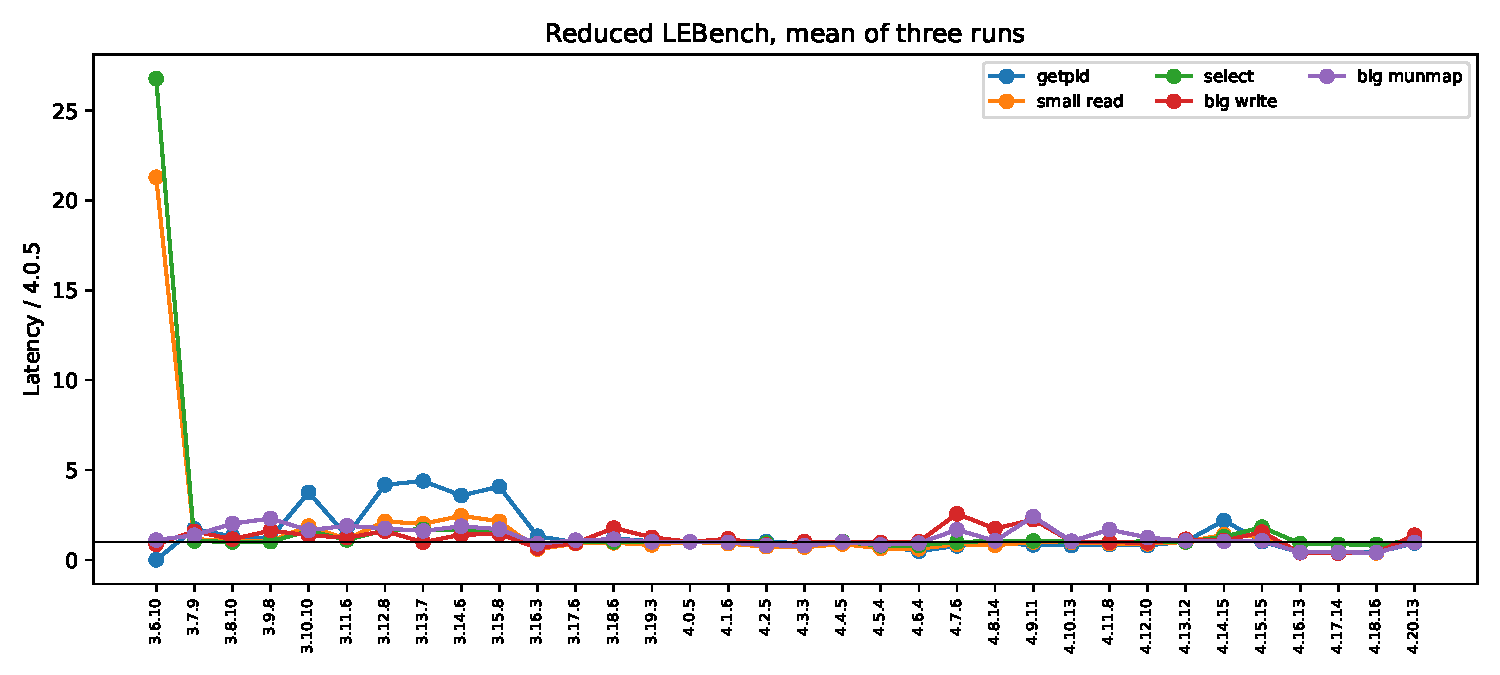
\includegraphics[width=\linewidth]{generated/relative_latency.pdf}
\caption{延迟除以本客户机上 4.0.5 的结果。横线 1 是论文的基线内核。纵轴文字仍是英文，因为图由同一份汇总脚本画出。}
\label{fig:rel}
\end{figure}
}{}

\section{分析}

论断 1 看的是相对 4.0 的变化方向，不是绝对纳秒数。这里的绝对时间不是论文里的时间：客户机只有两个很慢的虚拟 CPU，磁盘是虚拟磁盘，迭代次数也更短，所以一个离群点就会挪动 K-best 窗口。表~\ref{tab:nopti} 里的标准差经常占均值的很大一部分。小于标准差的差值不能当作证据。下面的结论使用这条规则：只有当更晚内核的“均值 $\pm$ 标准差”区间整个落在 4.0.5 的区间之上时，才把它算作更慢。

按这条规则，论断 1 在这台客户机上\textbf{不成立}。627 项更晚内核的测量里，只有 271 项（43\%）的均值高于 4.0.5，只有 117 项同时满足区间不重叠且均值更高。论文说的“大多数测试更慢，而且很多至少慢 50\%”对不上这张表：627 项里只有 76 项（12\%）的均值至少高 50\%。拆到那 19 个更晚的内核上，getpid 有 5 个均值更高，有 9 个区间明显更快；fork 的更高均值个数是 0。论文把大块写当作变快的例外，它在 19 个内核里有 11 个均值更高，但只有 1 个区间超出了噪声。和 Linux 3.0 的比较是\textbf{无法判断}：3.0.7 到 3.5.4 从未连上 sshd，这台客户机上没有 3.0 基线。

论断 2 只碰到了 \texttt{nopti} 这一个开关。论文的 KPTI 结果需要一颗会为页表隔离付出代价的 CPU。i7-13700H 报告它不会。这个开关仍然改变了 \texttt{fork}，所以命令行不是空操作，但它没有复现出“KPTI 让 \texttt{getpid}、读和 recv 变慢”。论断 2 的这一部分在这里\textbf{不成立}。

论断 3 没有测。本仓库里没有 Redis、Apache 或 Nginx 的数字，所以应用层面的论断\textbf{无法判断}。

这次运行给不出原服务器上的热力图、十一项消融，以及应用程序的加速。到不了 sshd 的内核记在 \texttt{results/kernels/progress.log} 的启动失败里，不给它们填一个延迟。

\section{扩展：把 getpid 改成批量计时}
\label{sec:batch}

精简套件在两次 \texttt{clock\_gettime} 之间只调用一次 \texttt{getpid}。在 4.0.5 上，空跑的 \texttt{ref} 是 156 $\pm$ 64 ns，\texttt{getpid} 是 245 $\pm$ 0 ns，计时器占了这个数字的很大一部分。扩展实验只改这一项。\texttt{course/OS\_Eval\_batched.c} 从精简源生成，把 \texttt{getpid} 改成一次计时 1{,}000 次调用再除以 1{,}000。K-best、\texttt{BASE\_ITER}、编译选项和其它测试都不变。每个内核把新二进制跑了三次。日志在 \texttt{results/batching/<版本>/run\{1,2,3\}.csv}。

\begin{table}[ht]
\centering
\caption{三次 K-best 的均值 $\pm$ 样本标准差。单次一列来自精简扫描，批量一列是上面这一处改动。}
\label{tab:batch}
\begin{tabular}{@{}lrr@{}}
\toprule
内核 & 单次 getpid & 批量 getpid \\
\midrule
4.0.5 & 245 $\pm$ 0 ns & 129 $\pm$ 0 ns \\
4.4.0-210 & 314 $\pm$ 39 ns & 127 $\pm$ 40 ns \\
\bottomrule
\end{tabular}

\end{table}

在 4.0.5 上，批量之后每次调用是 129 ns，单次是 245 ns，两个区间不重叠。同一天这份二进制的空跑时钟对是 132 $\pm$ 19 ns，和批量后的每次调用接近。在 4.4.0-210 上，单次均值是 314 ns，区间整个在 4.0.5 之上。批量之后两个均值是 127 ns 和 129 ns，区间重叠。这两个内核之间看起来的 \texttt{getpid} 变慢，在这一处改动之后没有了。批量二进制上的 \texttt{small read} 仍落在单次结果的波动里（4.0.5：813 $\pm$ 72 ns，对照 726 $\pm$ 73 ns），所以套件的其余部分没有跟着这次修改一起变。

\section{另一份实现}
\label{sec:rewrite}

仓库外面还有一棵从头重写的 LEBench。它是一组 Linux C 程序（\texttt{src/bench\_*.c}），配一份结果表为空的中文报告。上面的数字没有用它。里面有用的是 K-best 的说明和操作列表。测量本身不能拿来替换 \texttt{OS\_Eval}：

\begin{itemize}
\item 它用 \texttt{rdtsc} 计时，而且没有把指令流串行化。在这台 VirtualBox 客户机上，TSC 相对宿主机的偏移不稳定，所以作者的代码用 \texttt{clock\_gettime}。
\item \texttt{select} 在计时区间里分配并填满描述符位图，数字里包含了分配器的开销。
\item 上下文切换是一整段循环再除以迭代次数。这是平均值，不是论文里反复试验的 K-best，也没有把优先级调到 $-20$。
\item 缺页样本会摸每一页，再除以页数。第一次缺页时，fault-around 会把相邻页一起填上，所以同一次样本里后面的触摸常常不是缺页。\texttt{OS\_Eval} 只给一次触摸计时。
\item 迭代次数、空系统调用的选法，以及没有第三次进程运行，都和论文、也和课程要求不一样。
\item 它只在 Windows 上对着占位头文件编译过，没有在 Linux 上执行。那份报告自己也是这么写的。
\end{itemize}

让课程这棵树更接近论文的改动在 \texttt{course/} 和 \texttt{scripts/vm\_kernel\_sweep.py}：调用作者的函数，保留 K-best，重复三次，建好 \texttt{OS\_Eval} 拼到 \texttt{LEBENCH\_DIR} 后面的 Unix 套接字目录，并用 \texttt{grub-reboot} 启动，而不是把 GRUB 装到一个分区上。

\section{结论}

这次复现是部分完成的。作者列出的 41 个内核里，34 个把精简基准跑了三次。在这些日志上，“4.0 之后大多数核心操作变慢了”这一条不成立；在一颗不受 Meltdown 影响的 CPU 上，\texttt{nopti} 也没有复现出 KPTI 变慢。在 4.0.5 和 4.4.0-210 上把 \texttt{getpid} 改成批量计时之后，报告的每次调用大约少了一半，两个内核之间的变慢也不见了，所以原来那一行主要是计时器。应用程序一节和十一项原因的消融没有复现。实际的教训是：把微基准抄到一个新计时器上，以及一个装得上却启动不了的内核镜像，都会安静地失败。前者仍然会打出一个数字，后者则根本走不到打印数字的那一步。日志必须能看出发生的是哪一种。

\section*{贡献说明}

邹浩宇（5260000157）导入了 \texttt{6aa7801} 的 LEBench，安装了 Ubuntu 16.04.6 客户机，编写了精简运行程序和重启驱动，收集了 \texttt{results/kernels/} 下的日志，测量了 \texttt{results/batching/} 下的批量 \texttt{getpid}，并撰写了本报告和幻灯片。这项工作的提交说明使用该学号和姓名。

\section*{AI 使用说明}

Cursor 里的 AI 编程助手起草了运行程序、重启脚本、本报告和幻灯片，并操作了虚拟机。内核包、基准程序源代码和延迟数字来自 LEBench 作者以及客户机日志。助手没有编造测量值。

\begin{thebibliography}{9}
\bibitem{ren2019lebench}
Xiang (Jenny) Ren, Kirk Rodrigues, Luyuan Chen, Camilo Vega, Michael Stumm, and Ding Yuan.
An Analysis of Performance Evolution of Linux's Core Operations.
In \emph{Proceedings of SOSP}, 2019.
\url{https://doi.org/10.1145/3341301.3359640}
\end{thebibliography}

\end{document}
